\documentclass[12pt,oneside,slovak,a4paper]{article}

\usepackage[slovak]{babel}
\usepackage[utf8]{inputenc}
\usepackage{amsmath}
\usepackage{amsfonts}
\usepackage{amssymb}
\usepackage{graphicx}
\usepackage{cite}
\usepackage[IL2]{fontenc} % lepšia sadzba písmena Ľ než v T1
\usepackage{pdfpages}
\usepackage{url} % príkaz \url na formátovanie URL
\usepackage[hidelinks]{hyperref} % odkazy v texte budú aktívne (pri niektorých triedach dokumentov spôsobuje posun textu)
\usepackage[left=2cm,right=2cm,top=2cm,bottom=2cm]{geometry}
\usepackage{float}
\usepackage[normalem]{ulem}
\useunder{\uline}{\ul}{}
\usepackage{titling}
\usepackage{xcolor}
\usepackage{lipsum}
\usepackage{setspace}
\usepackage{blindtext}
\usepackage{caption}
\usepackage{tabularx}
\usepackage[numbers]{natbib}
\usepackage{listings} % for text/code highlighting

% riadkovanie 1.5
\begin{document}
\linespread{1.5}\selectfont

\begin{titlepage}
	\centering
    {\Large Slovenská technická univerzita v Bratislave\par}
    {\Large Fakulta informatiky a informačných technológií\par}
	\vspace{7cm}
	{\huge\bfseries Voľne šíriteľné nástroje na obnovu zmazaných súborov\par}
	\vspace{0.5cm}
    {\Large \textsc{Princípy informačnej bezpečnosti}\par}
    \vspace{1cm}
	{\Large\itshape Marek Čederle\par}
    {\small\texttt{xcederlem@stuba.sk}\par}
	\vfill

	{\large \today\par}
\end{titlepage}


\tableofcontents
\vspace*{\fill}
\pagebreak

% ----------------- 1. kapitola -----------------

% vsetky zdroje z literatura.bib aby sa zobrazili bez citovania
\nocite{*}

\section{Špecifikácia projektu}
V mojom projekte sa budem venovať analýze súborových systémov pre operačné systémy Windows a GNU+Linux. Bude sa jednať o súborové systémy typu NTFS a ext ale spomeniem aj dodnes veľmi používané FAT32 a exFAT ktoré sa používajú na prenosných médiách. Každý súborový systém by som chcel opísať s tým, že uvediem jeho výhody a nevýhody prípadné porovnanie s ďalšími spomenutými súborovými systémami.

Budem sa zaoberať aj tým, ako správne naformátovať disk (prepísať ho náhodnými dátami alebo samými nulami) aby pri jeho predaji sa z bezpečnostných dôvodov nedalo zistiť čo sa na ňom pred tým nachádzalo. Je to z dôvodu že pri mazaní dát z disku sa vlastne tieto dáta reálne nemažú. Dáta na disku zostanú, len sa z tabuľky záznamov zahodí záznam kde sa súbor nachádza a potom keď sa zapisuje na disk tak operačný systém vie, že môže na toto miesto zapisovať. 

Taktiež sa budem zaoberať analýzou nástroja na obnovu zmazaných súborov s názvom testdisk. Vysvetlím, prečo som si vybral práve tento nástroj. S týmto nástrojom budem následne experimentovať. Experimenty budú spočívať v tom, že si naformátujem disk a vytvorím na ňom nejaké partície podľa typu daného súborového systému. Následne naň uložím rôzne typy súborov. Budú sa tam nachádzať fotky, textové súbory, archívy, atď. Potom vymažem nejaké z týchto súborov, ale na disk ďalej nič nezapíšem, aby sa nezačali prepisovať dané miesta na disku inými súbormi. Následne vyskúšam nástroj na obnovu zmazaných súborov (testdisk) či zvládne tieto súbory obnoviť. Tento experiment zopakujem s tým, že po zmazaní ďalších súborov zapíšem na disk zase nové súbory a vyskúšam použiť nástroj na obnovu či dokáže aj po takejto akcii obnoviť súbory. Ďalší experiment bude spočívať v zmazaní celej partície a jej následnej obnove týmto nástrojom. V neposlednom rade ukážem, že po správnom formátovaní disku sa nebudú dať dáta obnoviť. Na záver budem prezentovať výsledky experimentov.
\subsection{Progress report č.1}
V prvom progress reporte vypracujem teoretickú časť, ktorú som na začiatku uviedol. To znamená popísanie rôznych typov súborových systémov a nástrojov na obnovu súborov. V neposlednom rade uvediem ako z bezpečnostného hľadiska správne ``zmazať'' súbory na disku respektíve ako ho naformátovať tak, aby sa z neho minulé dáta nedali prečítať.

\subsection{Progress report č.2}
V tomto progress reporte sa budem zameriavať na praktickú/experimentálnu časť. To znamená, že sa pokúsim vykonať všetky vyššie spomenuté experimenty. Na záver budem pracovať na celkovej úprave finálneho dokumentu.

\subsection{Ciele projektu}
Cieľom tohto projektu je získať informácie z oblasti súborových systémov a vykonať rôzne experimenty s nástrojmi na obnovu údajov. Keďže sa jedná o predmet Princípy informačnej bezpečnosti, tak cieľom je poukázať na dopady neformátovania respektíve neefektívneho ``ničenia'' súborov na bezpečnosť.

% ----------------- 2. kapitola -----------------

\section{Súborové systémy}
Súborový systém je metóda a dátová štruktúra, ktorú operačný systém používa na riadenie spôsobu ukladania a načítavania dát. Bez súborového systému by dáta umiestnené na pamäťovom médiu boli jedným veľkým zväzkom dát bez možnosti určiť, kde končí jeden súbor a začína ďalší, alebo kde sa nachádza, keď je potrebné ho načítať. Rozdelením dát na časti a pomenovaním každej časti sa dáta ľahko izolujú a identifikujú. Každá skupina dát sa nazýva súbor.

\subsection{FAT - File Allocation Table}
FAT je súborový systém vyvinutý pre osobné počítače. Pôvodne vyvinutý v roku 1977 na použitie na disketách, neskôr bol prispôsobený na použitie na pevných diskoch a iných zariadeniach. Často je z dôvodov kompatibility podporovaný súčasnými operačnými systémami pre osobné počítače a mnohými mobilnými zariadeniami a ``embed'' systémami. FAT ako taký je už v dnešnej dobe nepoužívaný, ale jeho odnože (FAT32, exFAT) sa doteraz používajú napríklad v prenosných médiách ako USB kľúče, SD karty a podobne.

\subsubsection{FAT32}
Najpokročilejšia verzia súborového systému FAT je FAT32. S FAT32 sa Microsoft snažil prekonať obmedzenia FAT16 a prispôsobiť sa väčším možným partíciám. Existuje už od Windowsu 95 a naďalej zostáva populárny, pretože je vysoko kompatibilný s väčšinou operačných systémov (GNU+Linux, MAC) a prenosných zariadení. FAT32 podporuje súbory do 4 GB a partície s maximálnou veľkosťou 2 TB. Používa sa prevažne pre EFI partície a prenosné médiá s kapacitou do 32GB.

\subsubsection{Štruktúra FAT a FAT32}
Novo naformátovaný disk s FAT vyzerá nasledovne:

\begin{figure}[H]
	\centering
	\captionsetup{justification=centering,margin=2cm}
	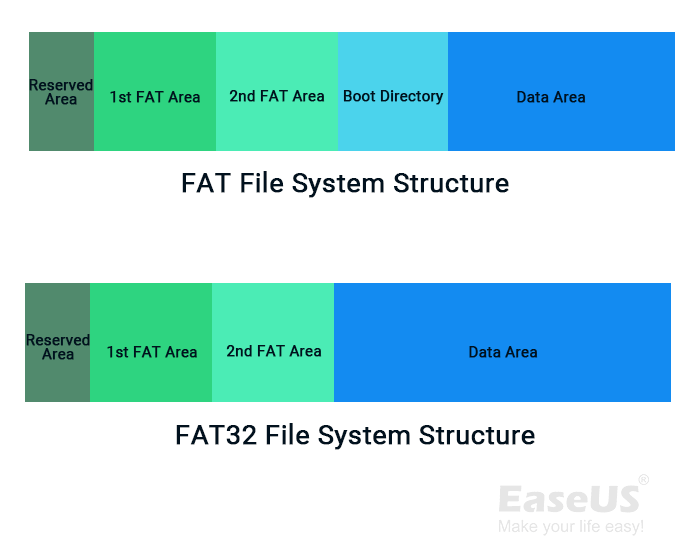
\includegraphics[width=\linewidth]{./images/file_system_structure/fat-file-system-structure.png}
	\centering
	\caption{Štruktúra súborového systému FAT a FAT32 \\ Zdroj: https://www.easeus.com/diskmanager/file-system.html}
\end{figure}

\begin{spacing}{1.0}
\begin{itemize}
	\item Reserved Area
		\begin{itemize}
			\item Obsahuje boot sector, BPB (BIOS Parameter Block) a celkovo informácie potrebné pre bootovanie a súborový systém.
		\end{itemize}
	\item 1st FAT Area
		\begin{itemize}
			\item FAT tabuľka obsahujúca informácie o súboroch a ich umiestnení na disku.
		\end{itemize}
	\item 2nd FAT Area
		\begin{itemize}
			\item Obsahuje kópiu FAT tabuľky.
		\end{itemize}
	\item Boot Directory
		\begin{itemize}
			\item Niekedy sa nazýva aj Root Directory. Používa sa iba v derivátoch FAT12 a FAT16. Obsahuje informácie o súboroch, ktoré sa nachádzajú priamo v koreňovom adresári.
		\end{itemize}
	\item Data Area
		\begin{itemize}
			\item Obsahuje samotné dáta súborov.
		\end{itemize}
\end{itemize}
\end{spacing}

\subsubsection{exFAT - Extensible File Allocation Table}
exFAT je súborový systém predstavený spoločnosťou Microsoft v roku 2006 a optimalizovaný pre flash pamäte, ako sú USB flash disky a SD karty. exFAT bol proprietárny do 28. augusta 2019, kedy Microsoft zverejnil jeho špecifikáciu. Microsoft však stále vlastní patenty na niekoľko častí svojho dizajnu. To spôosobilo rozšírenie jeho podpory medzi rôzne operačné systémy.

exFAT možno použiť tam, kde NTFS nie je vhodným riešením (kvôli vysokej réžii\footnote{angl. overhead}), ale kde je potrebná podpora súborov väčších ako 4 GB. Podporuje rádovo väčšiu veľkosť súborov ako FAT32 (ExaByty).

exFAT bol prijatý SD Association ako predvolený súborový systém pre karty SDXC väčšie ako 32 GB.

Windows 8 a novšie verzie natívne podporujú bootovanie z exFAT.

\subsubsection{Štruktúra exFAT}
Novo naformátovaný disk s exFAT vyzerá nasledovne:

\begin{figure}[H]
	\centering
	\captionsetup{justification=centering,margin=2cm}
	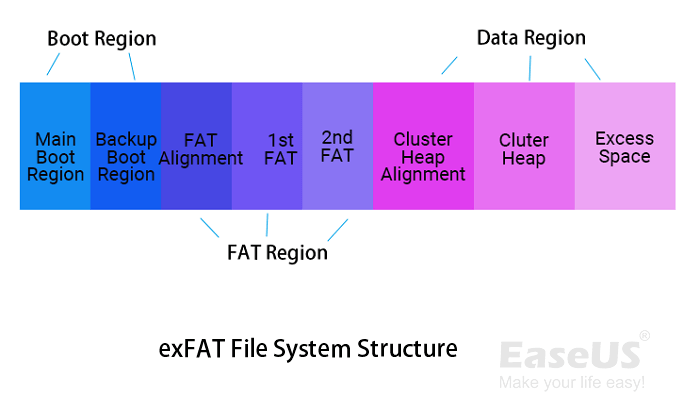
\includegraphics[width=\linewidth]{./images/file_system_structure/exfat-file-system-structure.png} %scale=0.64
	\centering
	\caption{Štruktúra súborového systému exFAT \\ Zdroj: https://www.easeus.com/diskmanager/file-system.html}
\end{figure}

\begin{spacing}{1.0}
\begin{itemize}
	\item Boot Region
		\begin{itemize}
			\item Main Boot Region
			\begin{itemize}
				\item Informácie potrebné pre bootovanie.
			\end{itemize}
		\item Backup Boot Region
			\begin{itemize}
				\item Záloha Main Boot Region.
			\end{itemize}
		\end{itemize}

	\item FAT Region
		\begin{itemize}
			\item FAT Alignment
				\begin{itemize}
					\item FAT offset a veľkosť.
				\end{itemize}
			\item 1st FAT
				\begin{itemize}
					\item FAT tabuľka obsahujúca informácie o súboroch a ich umiestnení na disku.
				\end{itemize}
			\item 2nd FAT
				\begin{itemize}
					\item Záloha FAT tabuľky.
				\end{itemize}
		\end{itemize}

	\item Data Region
		\begin{itemize}
			\item Cluster Heap Alignment
				\begin{itemize}
					\item Cluster heap offset a veľkosť.
				\end{itemize}
			\item Cluster Heap
				\begin{itemize}
					\item Obsahuje samotné dáta súborov.
				\end{itemize}
			\item Excess Space
				\begin{itemize}
					\item Zvyšok priestoru na disku.
				\end{itemize}
		\end{itemize}
\end{itemize}
\end{spacing}

\subsubsection{Výhody a nevýhody FAT32 a exFAT}

% tabulka pre FAT32
\begin{table}[H]
\begin{tabularx}{\textwidth}{|X|X|}
\hline
\multicolumn{2}{|c|}{\textbf{FAT32}} \\ \hline
\multicolumn{1}{|c|}{\textbf{Výhody}} & \multicolumn{1}{c|}{\textbf{Nevýhody}} \\ \hline
Vysoko kompatibilný s rôznymi operačnými systémami. & Nedokáže uložiť súbor, ktorý je väčší ako 4GB. \\ \hline
Je kompatibilný s väčšinou prenosných úložných zariadení. & Nemá natívne šifrovanie súborov a chýbajú mu prístupové povolenia prítomné v moderných súborových systémoch. \\ \hline
& FAT32 je pomalší na čítanie a zápis dát v porovnaní s modernými súborovými systémami. \\ \hline
\end{tabularx}
\centering
\captionsetup{justification=centering,margin=2cm}
\caption{Výhody a nevýhody súborového systému FAT32 \\ Zdroj: https://superops.com/ntfs-vs-fat32}
\end{table}

% tabulka pre exFAT
\begin{table}[H]
\begin{tabularx}{\textwidth}{|X|X|}
\hline
\multicolumn{2}{|c|}{\textbf{exFAT}} \\ \hline
\multicolumn{1}{|c|}{\textbf{Výhody}} & \multicolumn{1}{c|}{\textbf{Nevýhody}} \\ \hline
Podporuje súbory väčšie ako 4GB. & Absencia žurnálovania a kompresie dát. \\ \hline
Je predvoleným systémom na SD kartách s vysokou kapacitou & Nemá podporu pre staršie operačné systémy bez špeciálnych ovladačov. \\ \hline
Veľkosť partície je v podstate neobmedzená. & Nemá natívnu podporu pre šifrovanie dát. \\ \hline
Efektívenejší ako FAT32. & Nie je efektívnejší ako NTFS alebo ext. \\ \hline
Podpora všetkých majoritných operačných systémov. & Nie je vhodný pre viac-používateľské aplikácie z dôvody vyššej fragmentácie. \\ \hline
\end{tabularx}
\centering
\captionsetup{justification=centering,margin=2cm}
\caption{Výhody a nevýhody súborového systému exFAT \\ Zdroj: https://www.profolus.com/topics/exfat-advantages-disadvantages-extensible-fat/}
\end{table}

\subsection{NTFS - New Technology File System}
NTFS je proprietárny súborový systém vytvorený spoločnosťou Microsoft. Bol uvedený s vtedy novým operačným systémom Windows NT\footnote{New Technology} v roku 1993. Vtedy nahradil dovtedy veľmi používaný súborový systém FAT. NTFS je predovšetkým určený pre pevné disky HDD\footnote{Hard Disk Drive} a neskôr aj pre SSD\footnote{Solid State Drive}. Je však možné ho použiť aj na prenosové média typu USB kľúč a podobne.

Súborový systém NTFS prináša kombináciu vyššej rýchlosti, väčšej spoľahlivosti a kompatibility oproti súborovému systému FAT, ktorý bol jeho predchodcom v ére operačného systému MS DOS. Natívne podporuje šifrovanie a kompresiu súborov. Podporuje aj veľmi veľké súbory a partície.

Ide o žurnálový súborový system, čo znamená, že všetky zmeny na disku sú zaznamenané v tzv. žurnáli. V prípade výpadku napájania alebo zlyhania systému je možné rýchlo obnoviť dáta na disku.

\subsubsection{Štruktúra NTFS}
Novo naformátovaný disk s NTFS vyzerá nasledovne:

\begin{figure}[H]
	\centering
	\captionsetup{justification=centering,margin=2cm}
	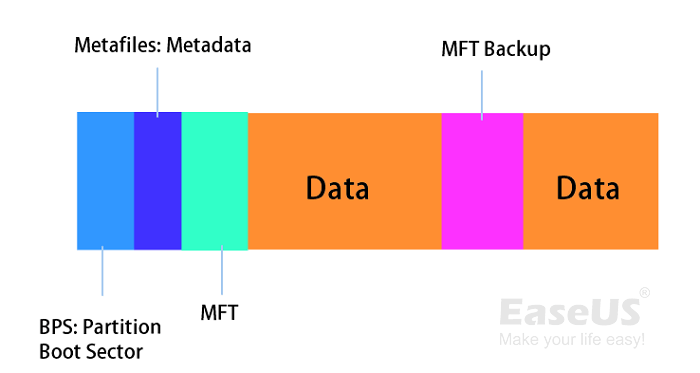
\includegraphics[width=\linewidth]{./images/file_system_structure/ntfs-file-system-structure.png}
	\centering
	\caption{Štruktúra súborového systému NTFS \\ Zdroj: https://www.easeus.com/diskmanager/file-system.html}
\end{figure}

% bulleted list plus riadkovanie iba na danu cas textu
\begin{spacing}{1.0}
\begin{itemize}
	\item Partition Boot Sector
		\begin{itemize}
			\item Obsahuje informácie potrebné pre bootovanie. Primárne sa jedná o BootStrap čo je vlastne malý program, ktorý ma za úlohu načítať operačný systém do pamäte.
		\end{itemize}
	\item Metadata
		\begin{itemize}
			\item Pomáhajú definovať a organizovať súborový systém, zálohovať kritické údaje súborového systému.
		\end{itemize}
	\item Master File Table (MFT)
		\begin{itemize}
			\item Obsahuje záznamy o všetkých súboroch a adresároch na disku. Je to v podstate ekvivalent FAT tabuľky.
		\end{itemize}
	\item Data
		\begin{itemize}
			\item Obsahuje samotné dáta súborov.
		\end{itemize}
	\item MFT Backup
		\begin{itemize}
			\item Obsahuje zálohu MFT tabuľky.
		\end{itemize}
\end{itemize}
\end{spacing}

\subsubsection{Bezpečnosť NTFS}
Ako som vyššie spomenul tak NTFS natívne podporuje šifrovanie súborov, priečinkov ale aj celých partícií. Súborový systém NTFS umožňuje nastaviť povolenia na prístup k niektorým lokálnym súborom a priečinkom. Inými slovami, dôverný súbor môžete nastaviť tak, aby bol pre niektorých iných používateľov nedostupný. Táto metóda sa nazýva riadenie úrovne prístupu (ACL).

\subsubsection{Výhody a nevýhody NTFS}

% tabulka s výhodami a nevýhodami NTFS
\begin{table}[H]
\begin{tabularx}{\linewidth}{|X|X|}
\hline
\multicolumn{1}{|c|}{\textbf{Výhody}} & \multicolumn{1}{c|}{\textbf{Nevýhody}} \\ \hline
Podporuje veľmi veľké súbory a nemá takmer žiadne reálne obmedzenie veľkosti oddielu. & Má uzatvorený zdrojový kód. \\ \hline
Poskytuje vylepšené zabezpečenie údajov pomocou funkcií riadenia úrovne prístupu a natívneho šifrovania. & Mac OS dokáže čítať jednotky naformátované v systéme NTFS, ale na systém NTFS je možné zapisovať iba prostredníctvom softvéru tretej strany. \\ \hline
Podporuje automatickú kompresiu súborov, čo umožňuje rýchlejší prenos súborov a väčší úložný priestor na disku. & Prenosné zariadenia, ako sú smartfóny so systémom Android a digitálne fotoaparáty, ho nepodporujú. \\ \hline
Umožňuje diskové kvóty, ktoré firmám poskytujú väčšiu kontrolu nad úložným priestorom. & Kompatibilita so systémami založenými na GNU+Linux síce existuje ale iba kvôli vôli softvérových inžinerov urobiť ovladače vďaka reverznému inžinierstvu. \\ \hline
Umožňuje používateľom sledovať pridané, upravené alebo odstránené súbory na disku. &  \\ \hline
Zameriava na konzistenciu súborového systému, takže v prípade výpadku napájania alebo zlyhania systému môžete rýchlo obnoviť svoje údaje. &  \\ \hline
\end{tabularx}
\centering
\captionsetup{justification=centering,margin=2cm}
\caption{Výhody a nevýhody súborového systému NTFS \\ Zdroj: https://superops.com/ntfs-vs-fat32}
\end{table}
% ------------- koniec tabulky -------------

\subsection{ext - Extended File System}
ext bol implementovaný v apríli 1992 ako prvý súborový systém vytvorený špeciálne pre jadro Linuxu. Má štruktúru metadát inšpirovanú tradičnými princípmi súborového systému Unix a navrhol ho Rémy Card, aby prekonal určité obmedzenia súborového systému MINIX. Bola to prvá implementácia, ktorá využívala virtuálny súborový systém (VFS\footnote{Virtual File System}), ktorého podpora bola pridaná do jadra Linuxu vo verzii 0.96c, a dokázala spracovať súborové systémy s veľkosťou až 2 GB.

ext bol prvým z radu rozšírených súborových systémov. V roku 1993 ho nahradili systémy ext2 a Xiafs, ktoré si istý čas konkurovali, ale ext2 zvíťazil vďaka svojej dlhodobej životaschopnosti: ext2 odstránil problémy ext, ako napríklad nemennosť inódov a fragmentáciu.

Ďaľej sa tento súborvý systém rozširoval a aktualizoval. Z tohto vznikli novšie verzie ext3 a ext4.

\subsubsection{ext4}
Podobne ako pri NTFS aj ext4 je tzv. žurnálový súborový systém. Je veľmi abstraktný čo je výhodou pre software pretože sa software developery nemusia zaoberať priveľa súborovým systémom a ich program bz mal fungovať na každom rovnako. Abstrakcia znamená že všetok hardware (disky, a pod.) sú v ext4 reprezentované ako súbor. Má až takú úroveň abstrakcia že vlastne všetko je v podstate súbor. Používa sa ako predvolený súborový systém pre disky na distribúciách založených na Debian a Ubuntu. Taktiež je spätne kombatibilný s ext3.

\subsubsection{Štruktúra ext4}
Novo naformátovaný disk s ext4 vyzerá nasledovne:

\begin{figure}[H]
	\centering
	\captionsetup{justification=centering,margin=2cm}
	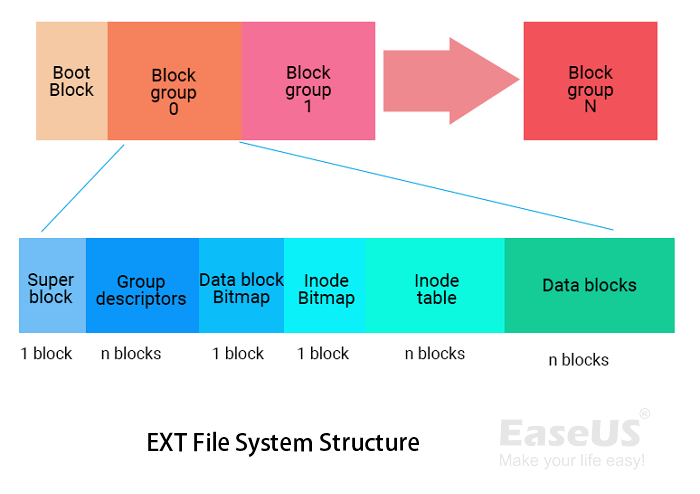
\includegraphics[width=\linewidth]{./images/file_system_structure/ext-file-system-structure.png}
	\centering
	\caption{Štruktúra súborového systému ext4 \\ Zdroj: https://www.easeus.com/diskmanager/file-system.html}
\end{figure}

% bulleted list plus riadkovanie iba na danu cas textu
\begin{spacing}{1.0}
\begin{itemize}
	\item Boot Block
		\begin{itemize}
			\item Informácie o bootovaní
		\end{itemize}
	\item Block group
		\begin{itemize}
			\item Super block
				\begin{itemize}
					\item Superblok sa nachádza na začiatku súborového systému a obsahuje metadáta o súborovom systéme vrátane jeho veľkosti, veľkosti bloku, počtu inódov a ďalších parametrov. Slúži ako hlavný riadiaci blok pre súborový systém
				\end{itemize}
			\item Group descriptors
				\begin{itemize}
					\item Skupinové deskriptory obsahujú metadáta pre danú skupinu
				\end{itemize}
			\item Data block Bitmap
				\begin{itemize}
					\item Sleduje status blokov pre danú skupinu
				\end{itemize}
			\item Inode Bitmap
				\begin{itemize}
					\item Sleduje status inodov pre danú skupinu
				\end{itemize}
			\item Inode Table
				\begin{itemize}
					\item Obsahujú metadáta a atribúty, čo sa týka oprávnení a ďaľších informácií pre každý súbor a adresár v danej skupine
				\end{itemize}
			\item Data blocks
				\begin{itemize}
					\item Obsahujú dané dáta
				\end{itemize}
		\end{itemize}
\end{itemize}
\end{spacing}

\subsubsection{Výhody a nevýhody ext4}

% tabulka s výhodami a nevýhodami ext4

\begin{table}[H]
\begin{tabularx}{\textwidth}{|X|X|}
\hline
\multicolumn{1}{|c|}{\textbf{Výhody}} & \multicolumn{1}{c|}{\textbf{Nevýhody}} \\ \hline
Podporuje najväčšiu individuálnu veľkosť súboru a veľkosť zväzku súborového systému. & Neposkytuje zabezpečenie dát. \\ \hline
Podporuje všetky znaky okrem NULL a '/.' & Ťažké vytvoriť snapshot na inom zväzku. \\ \hline
Môžete previesť súborový systém Ext3 na Ext4. & Využíva viacej miesta na disku. \\ \hline
Zahŕňa pokročilé funkcie ako rozšírenie, indexovanie adresárov, oneskorenú alokáciu a defragmentáciu. &  \\ \hline
Podporuje neobmedzený počet podadresárov. &  \\ \hline
Používa timestamp v nanosekundách. &  \\ \hline
Podporuje predalokácia pre rozsiahle súbory. &  \\ \hline
Podporuje viacnásobnú alokáciu blokov. &  \\ \hline
\end{tabularx}
\centering
\captionsetup{justification=centering,margin=2cm}
\caption{Výhody a nevýhody súborového systému Ext4 \\ Zdroj: https://www.easeus.com/partition-master/ext2-ext3-ext4-file-system-format-and-difference.html}
\end{table}

% ----------------- 3. kapitola -----------------

\section{Nástroje na obnovu údajov}
Existuje mnoho nástrojov na obnovu údajov. Či už ide o špecializované nástroje pre obnovu fotiek alebo multimediálnych súborov, alebo o univerzálne nástroje, ktoré dokážu obnoviť akékoľvek súbory. V tejto kapitole sa pozrieme na niektoré z nich.

\begin{spacing}{1.0}
\begin{itemize}
	\item Recuva
		\begin{itemize}
			\item Široko používaný a ľahko ovládateľný nástroj s pokročilými možnosťami skenovania pre rôzne typy súborov. Dostuoný pre platofrmu Windows.
		\end{itemize}
	\item PhotoRec
		\begin{itemize}
			\item Špecializovaný na obnovenie stratených obrázkov a multimediálnych súborov z rôznych úložných zariadení. Dostupný pre Windows, MacOS, Linux a ďalšie.
		\end{itemize}
	\item Testdisk
		\begin{itemize}
			\item Je od rovnakého vývojára ako PhotoRec. Dokáže obnoviť rôzne druhy súborov. Je univerzálny. Nielen obnovuje vymazané súbory, ale tiež pomáha opraviť tabuľku oddielov a boot sektory. Dostupný pre Windows, MacOS, Linux a ďalšie.
		\end{itemize}
	\item Disk Drill
		\begin{itemize}
			\item Veľmi podobný nástroj ako Recuva. Narozdiel od Recuvy, ktorá sa zaoberá skorej funkcionalitou, Disk Drill sa zameriava na používateľský zážitok (UX\footnote{User Experience}). Dostupný pre Windows, MacOS.
		\end{itemize}
\end{itemize}
\end{spacing}

\begin{figure}[H]
	\centering
	\begin{minipage}{.15\textwidth}
		\centering
        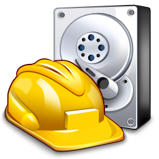
\includegraphics[width=\linewidth]{./images/tools-avatars/recuva.png}
		\captionsetup{justification=centering}
        \caption{Recuva}
    \end{minipage}\hfill
	\centering
	\begin{minipage}{.15\textwidth}
		\centering
        
\includegraphics[width=\linewidth]{./images/tools-avatars/photo_rec.png}
		\captionsetup{justification=centering}
        \caption{PhotoRec}
    \end{minipage}\hfill
    \centering
    \begin{minipage}{.15\textwidth}
        \centering
        
\includegraphics[width=\linewidth]{./images/tools-avatars/testdisk.png}
		\captionsetup{justification=centering}
        \caption{Testdisk}
    \end{minipage}\hfill
    \begin{minipage}{.15\textwidth}
        \centering
        
\includegraphics[width=\linewidth]{./images/tools-avatars/disk_drill.png}
		\captionsetup{justification=centering}
        \caption{Disk Drill}
    \end{minipage}\hfill
\end{figure}


\subsection{Testdisk}
Prečo som si vybral práve testdisk? Pretože je univerzálny, dokáže obnoviť rôzne druhy súborov. Taktiež vie opraviť tabuľku oddielov a boot sektory. Je crossplatform\footnote{Podporuje viacero operačných systémov} a zároveň je FOSS\footnote{Free \& Open Source Software --- zadarmo s voľne šíriteľným zdrojovým kódom}. Podporuje viacero typov partition table (MBR\footnote{Master Boot Record}, GPT\footnote{GUID Partition Table}). Zároveň podporuje viacero súborových systémov či už ide o FAT32, exFAT ale aj NTFS a ext. Má jednoduché rozhranie a nie je náročný na systém.


\section{Experimentovanie s nástrojom testdisk}

% fixnut ako toto znie a rozmiestnit obrazky

Najskôr bolo potrebné si pripraviť testovacie prostredie. Uvažoval som aj nad testovaním na fyzickom disku, ale keďže na mojom počítači mám operačný systém Windows a ten nedokáže pracovať s diskami, ktoré sú naformátované na ext, tak som sa rozhodol, že budem pracovať na virtuálnom stroji (VM\footnote{Virtual Machine}). Použil som program VirtualBox, ktorý je zadarmo. Na VM som nainštaloval vtedy najnovšiu verziu distribúcie Arch. Najprv som si nastavil prostredie aby sa mi lepšie pracovalo. Následne som si stiahol potrebné nástroje a dependencies. Potom som vytvoril virtuálne disky, ktorý som najskôr naformátoval a neskôr pripojil (mountol) do systému. Po tomto sa mohlo začať s experimentovaním.

Najpr som testoval tak, že som mal jeden disk o veľkosti 1 GB a mal 4 partície pre každý súborový systém, ktorému som sa chcel venovať (FAT32, exFAT, NTFS, ext4). Každá partícia mala veľkosť 200 MB. Neskôr kvôli komplikáciám s ext4 som skúsil aj samostatne jeden disk pre každý súborový systém.

Stiahol som si testovací súbor dostatočne veľký na to, aby pokrýval nadpolovičnú vačšinu z partície. Na toto som využil obrázok od NASA JWST\footnote{James Webb Space Telescope}, ktorý mal veľkosť 130MB.

\begin{figure}[H]
	\centering
	\captionsetup{justification=centering,margin=2cm}
	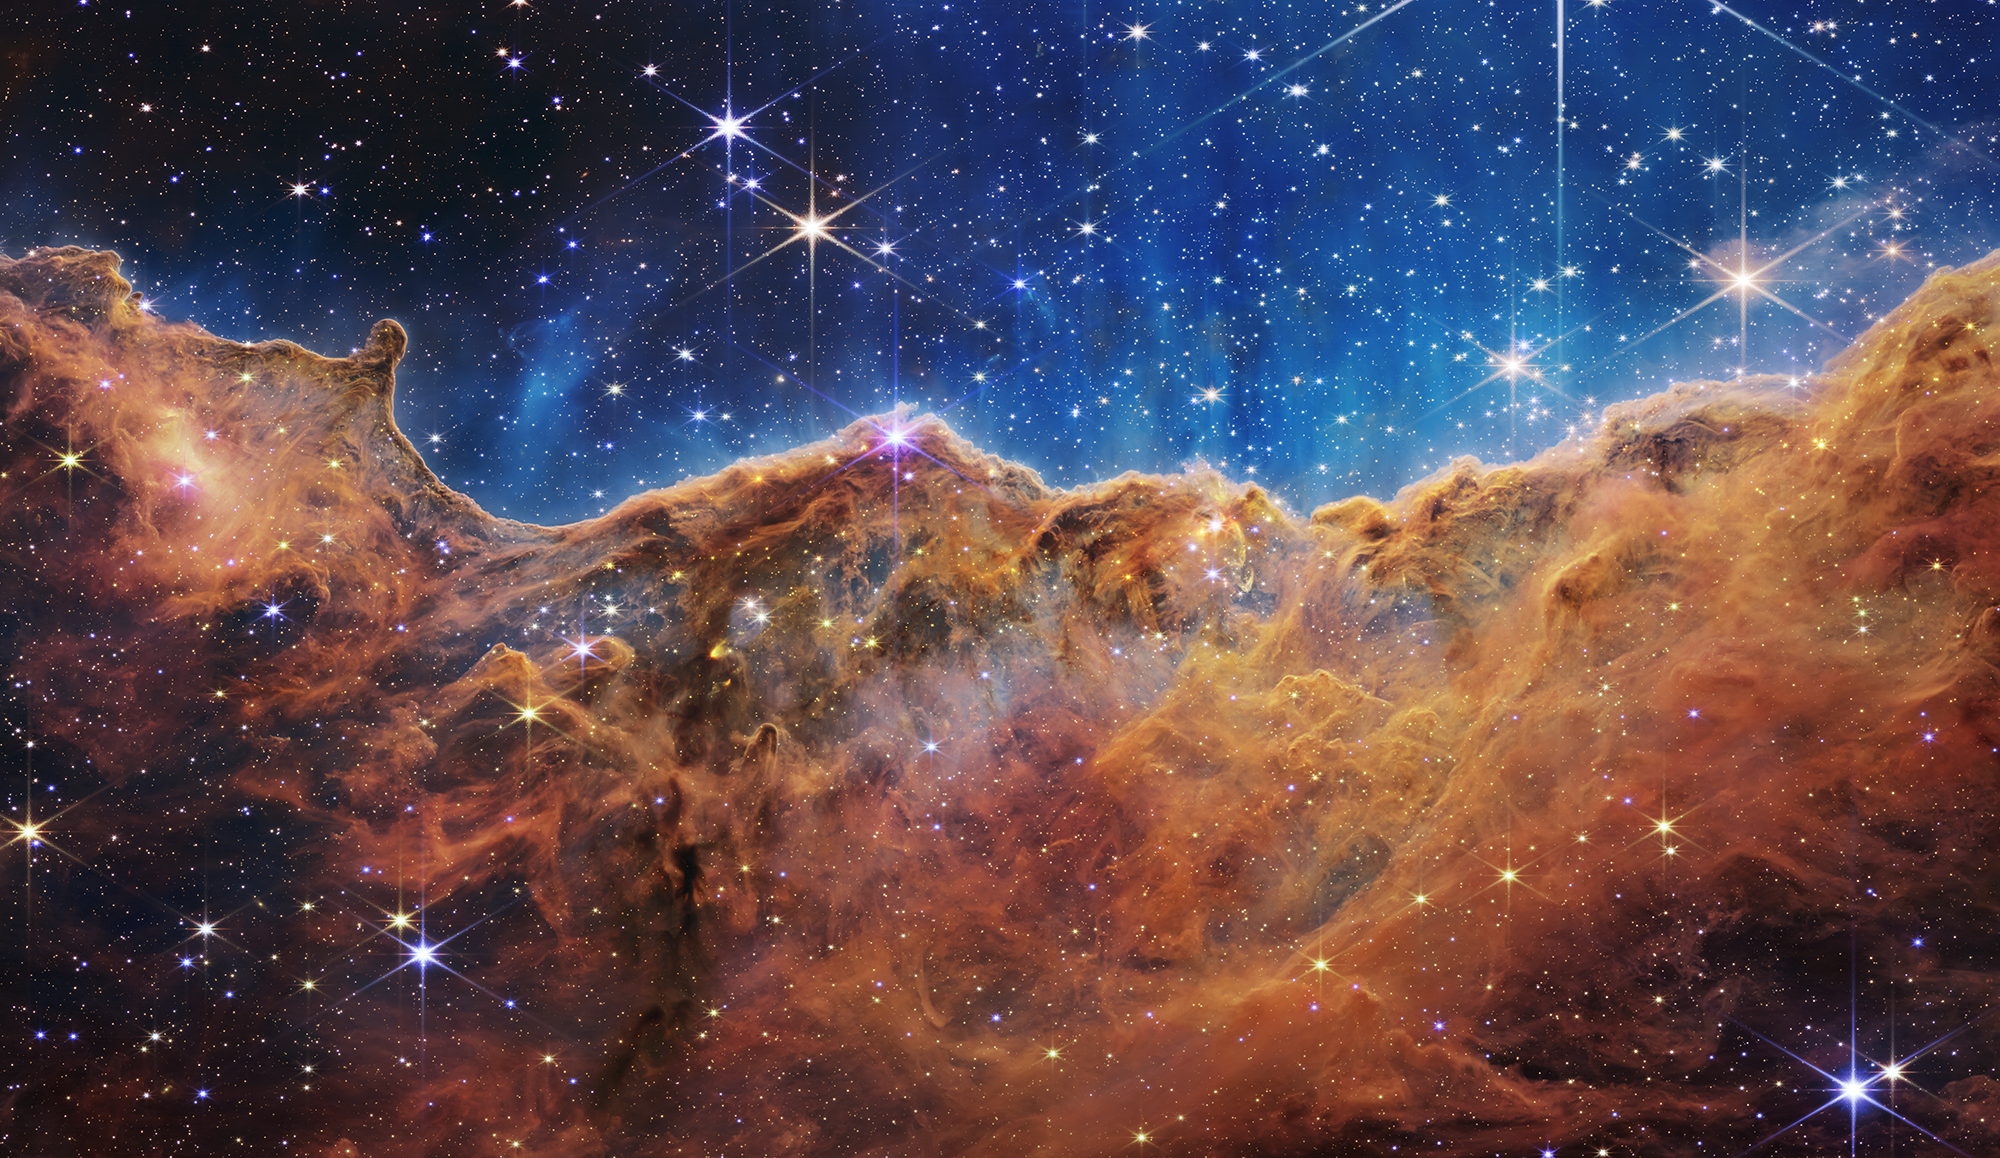
\includegraphics[width=\linewidth]{./images/testdisk_testing/NASA-JWST.png}
	\centering
	\caption{Testovací obrázok}
\end{figure}

\begin{figure}[H]
	\centering
	\captionsetup{justification=centering,margin=2cm}
	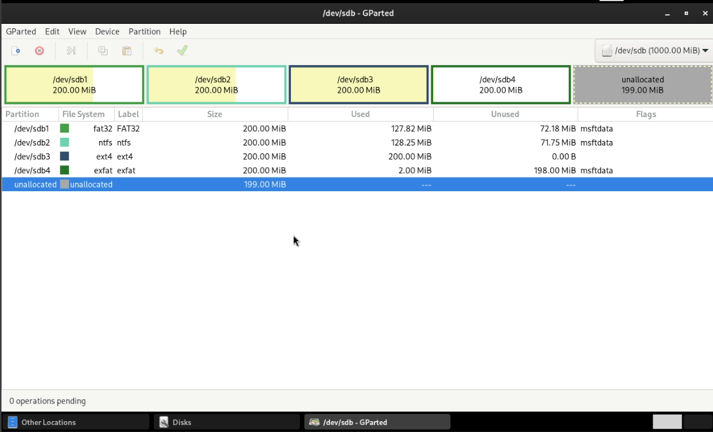
\includegraphics[scale=0.8]{./images/testdisk_testing/gparted-setup.png}
	\centering
	\caption{Gparted --- úvodné nastavenie diskov}
\end{figure}

\begin{figure}[H]
	\centering
	\captionsetup{justification=centering,margin=2cm}
	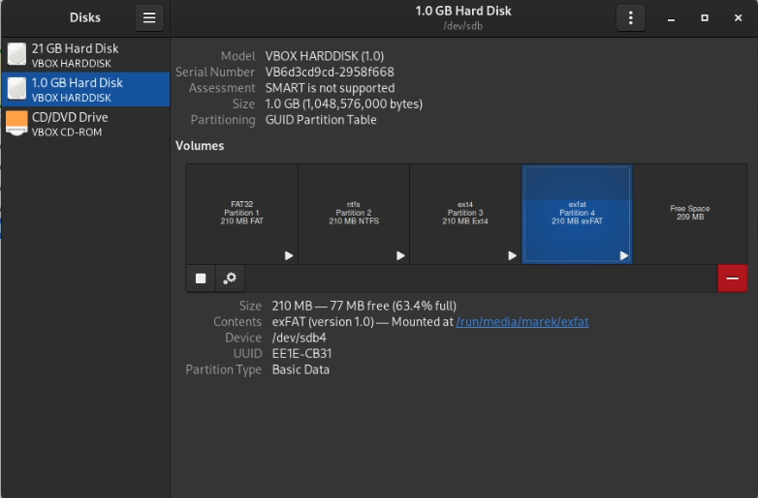
\includegraphics[scale=0.8]{./images/testdisk_testing/disk-mount-gnome-disks.png}
	\centering
	\caption{Mountnutie diskov/partícií pomocou Gnome Disks}
\end{figure}


\subsection{Zmazanie a obnova súborov}
Najskôr som naplnil všetky partície súborom.

\begin{figure}[H]
	\centering
	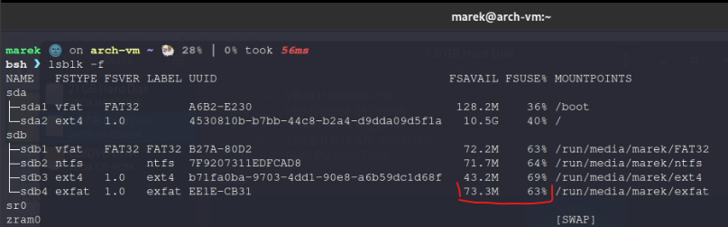
\includegraphics[scale=0.8]{./images/testdisk_testing/naplnenie_particii_lsblk.png}
	\centering
	\captionsetup{justification=centering,margin=2cm}
	\caption{Zobrazenie naplnených partícií --- lsblk}
\end{figure}

\begin{figure}[H]
	\centering
	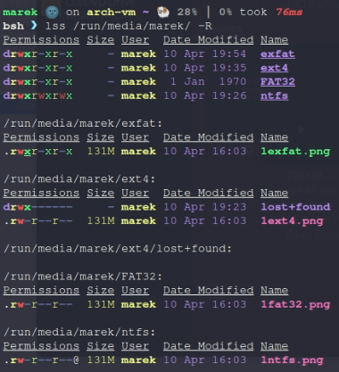
\includegraphics[scale=0.8]{./images/testdisk_testing/naplnenie_particii_lss.png}
	\centering
	\captionsetup{justification=centering,margin=2cm}
	\caption{Zobrazenie naplnených partícií --- ls}
\end{figure}


Následne som spustil nástroj testdisk v terminály.

\begin{figure}[H]
	\centering
	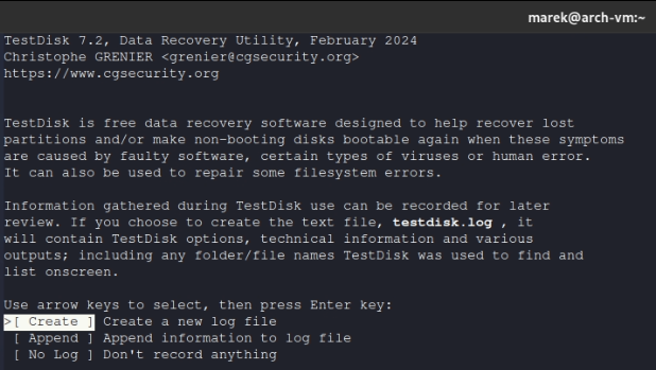
\includegraphics[scale=0.8]{./images/testdisk_testing/testdisk_UI.png}
	\centering
	\captionsetup{justification=centering,margin=2cm}
	\caption{Testdisk --- UI}
\end{figure}

Po vybratí typu logovania sa nám zobrazí obrazovka, kde si môžeme vybrať disk, s ktorým chceme pracovať.

\begin{spacing}{1.0}	
\begin{itemize}
	\item /dev/sda --- systémový disk
	\item /dev/sdb --- disk, ktorý som vytvoril pre testovanie
\end{itemize}
\end{spacing}


\begin{figure}[H]
	\centering
	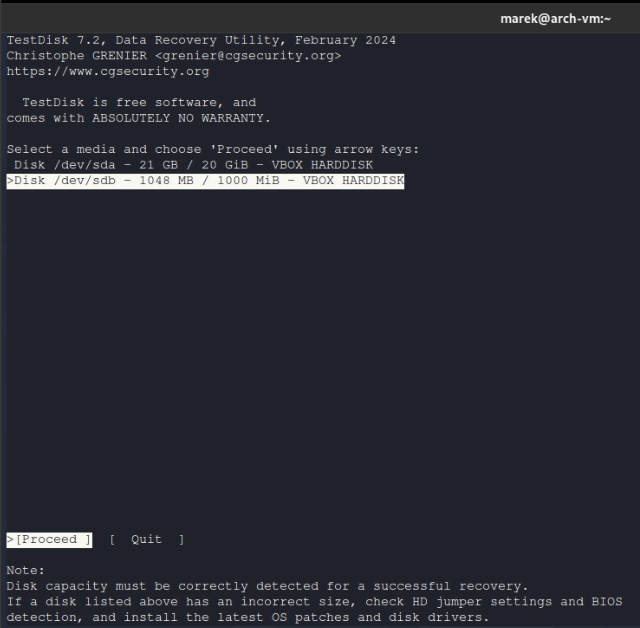
\includegraphics[scale=0.8]{./images/testdisk_testing/testdisk_choose_disk.png}
	\centering
	\captionsetup{justification=centering,margin=2cm}
	\caption{Testdisk --- výber disku}
\end{figure}

Následne nám nástroj automaticky zistí typ partition table. V prípade že nástroj zistí typ chybne, môžeme ho sami vybrať. Náš disk má partition table typu GPT, takže nástroj ho zistil správne a my sme možnosť potvrdili.

\begin{figure}[H]
	\centering
	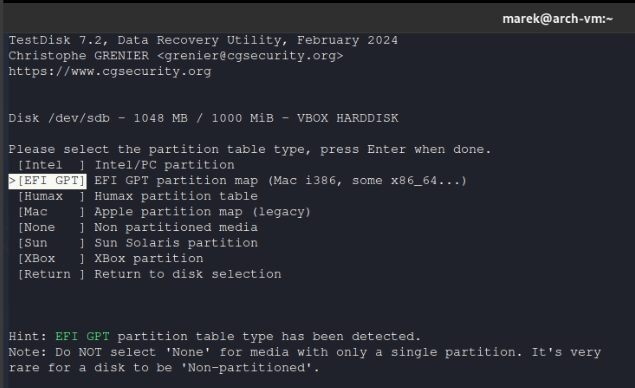
\includegraphics[scale=0.8]{./images/testdisk_testing/choose_partition_table.png}
	\centering
	\captionsetup{justification=centering,margin=2cm}
	\caption{Testdisk --- výber partition table}
\end{figure}

Po jeho vybratí sa nám zobrazilo menu na prácu s diskom. Pre nás podstatné budú možnosti ``Analyse'' a ``Advanced''.

\begin{spacing}{1.0}
	\begin{itemize}
		\item Analyse
			\begin{itemize}
				\item Táto možnosť nám umožní analyzovať disk a nájsť chyby súborového systému. Taktiež slúži na obnovu partícií.
			\end{itemize}
		\item Advanced
			\begin{itemize}
				\item Táto možnosť nám zobrazí zistené partície na disku. S ktorými budeme mocť ďalej pracovať.
			\end{itemize}
	\end{itemize}
\end{spacing}

Po vybratí možnosti ``Advanced'' nám nástroj zobrazí zistené partície na disku. Najskôr si vyberieme partíciu, s ktorou chceme pracovať a v dolnom menu si vyberieme čo chceme s danou partíciou robiť.

\begin{figure}[H]
	\centering
	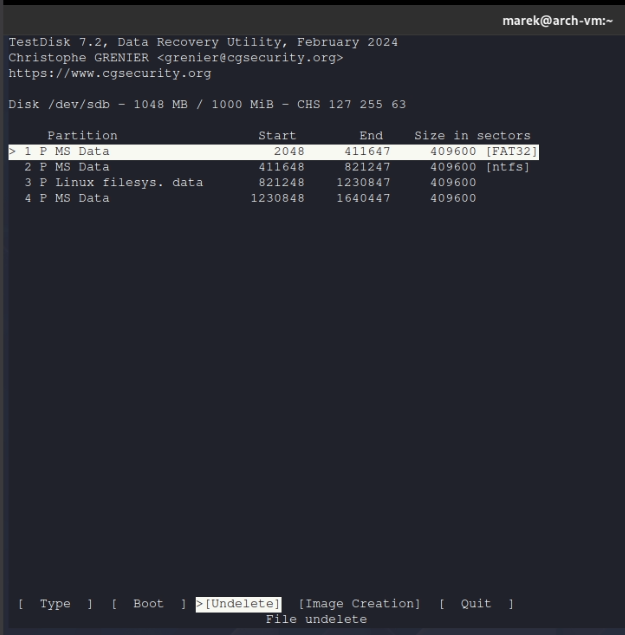
\includegraphics[scale=0.8]{./images/testdisk_testing/testdisk_choose_partition.png}
	\centering
	\captionsetup{justification=centering,margin=2cm}
	\caption{Testdisk --- výber partície}
\end{figure}

V našom prípade použijeme možnosť ``undelete'', ktorá umožnuje obnoviť zmazané súbory. Kedže sme zatiaľ nič nevymazali, tak nám zobrazí súbory a priečinky, ktoré sa tam nachádzajú podobne ako pri ``ls'' alebo ``dir''.

\begin{figure}[H]
	\centering
	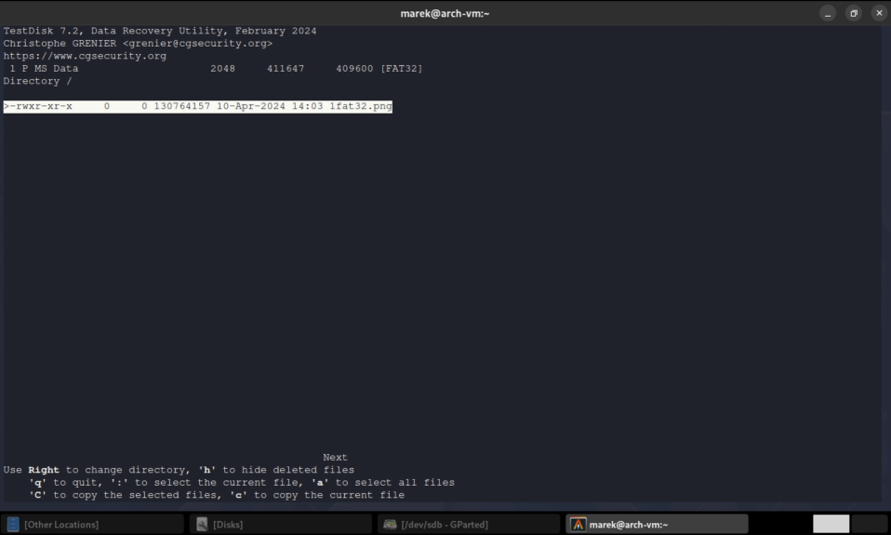
\includegraphics[scale=0.7]{./images/testdisk_testing/testdisk_list_files.png}
	\centering
	\captionsetup{justification=centering,margin=2cm}
	\caption{Testdisk --- zobrazenie súborov}
\end{figure}

Následne vypneme nástroj a zmažeme súbor z každej partície s tým, že zároveň ich vymažeme aj z koša.

\begin{figure}[H]
	\centering
	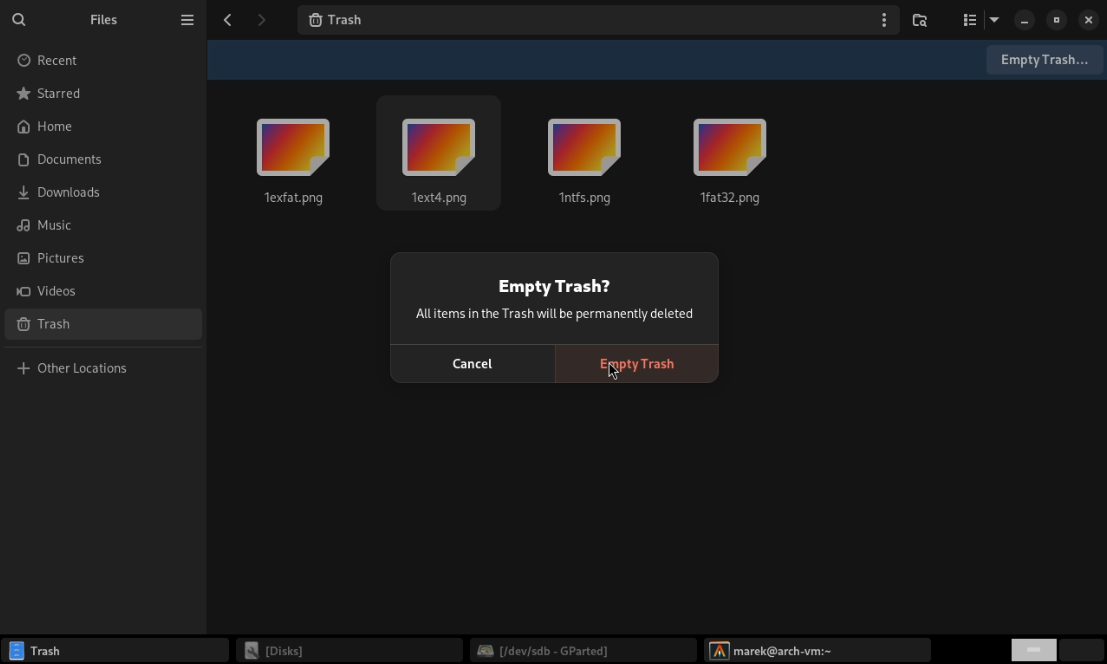
\includegraphics[width=\linewidth]{./images/testdisk_testing/file_deletion.png}
	\centering
	\captionsetup{justification=centering,margin=2cm}
	\caption{Vymazanie súborov}
\end{figure}

Potom si opäť spustíme nástroj testdisk s tým že urobíme rovnaké kroky ako boli pred chvíľou spomenuté. Následne si vyberieme možnosť ``undelete'' a nástroj nám zobrazí zmazaný súbor. Všimnime si, že teraz je súbor označený červenou farbou. Následne si ho zvolíme a stlačíme malé ``c'' na jeho skopírovanie.

\begin{figure}[H]
	\centering
	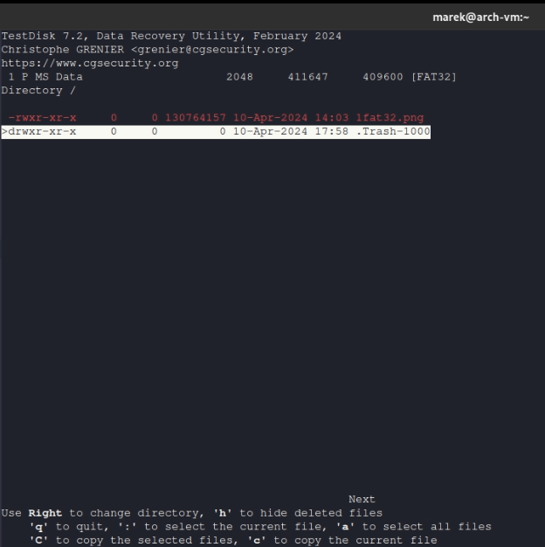
\includegraphics[scale=0.7]{./images/testdisk_testing/testdisk_deleted_file_recovery.png}
	\centering
	\captionsetup{justification=centering,margin=2cm}
	\caption{Testdisk --- obnova zmazaných súborov}
\end{figure}

Ďalej nám nástroj zobrazí možnosť kam chceme súbor skopírovať. Vyberieme si cestu a stlačíme veľké ``C''. Potom nám nástroj zobrazí informáciu o tom, či bol súbor úspešne skopírovaný.

\begin{figure}[H]
	\centering
	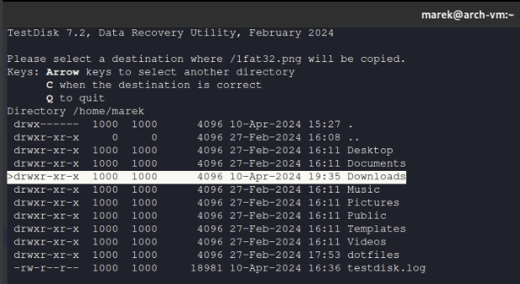
\includegraphics[scale=0.8]{./images/testdisk_testing/testdisk_deleted_file_recovery2.png}
	\centering
	\captionsetup{justification=centering,margin=2cm}
	\caption{Testdisk --- kopírovanie zmazaného súboru}
\end{figure}

Tento proces zopakujeme na všetkých partíciách nášho testovacieho disku.

\subsection{Zapísanie na miesto zmazaného súboru}
Po predošlom experimentovaní som stiahol iný obrázok z NASA JWST, ktorý mal veľkosť 172 MB. Uložil som ho na každú partíciu. Následne som ho vymazal, ale potom som na partície nahral ešte textový súbor, ktorý mal 150 MB aby prepísal pozostalé dáta o obrázku. Keď som sa pokúsil obnoviť obrázok, tak som síce našiel jeho záznam, ale keď som ho obnovil, tak jeho začiatok bol prepísaný textovým súborom. Týmto sme o dáta z obrázka prišli, pretože sa po obnovení nedal prezerať.

Tento proces som vizualizoval pomocou webu \url{https://binvis.io/}. Na obrázku je vidieť nepoškodený súbor vľavo a potom z polovice prepísaný súbor vpravo.

\begin{figure}[H]
	\centering
	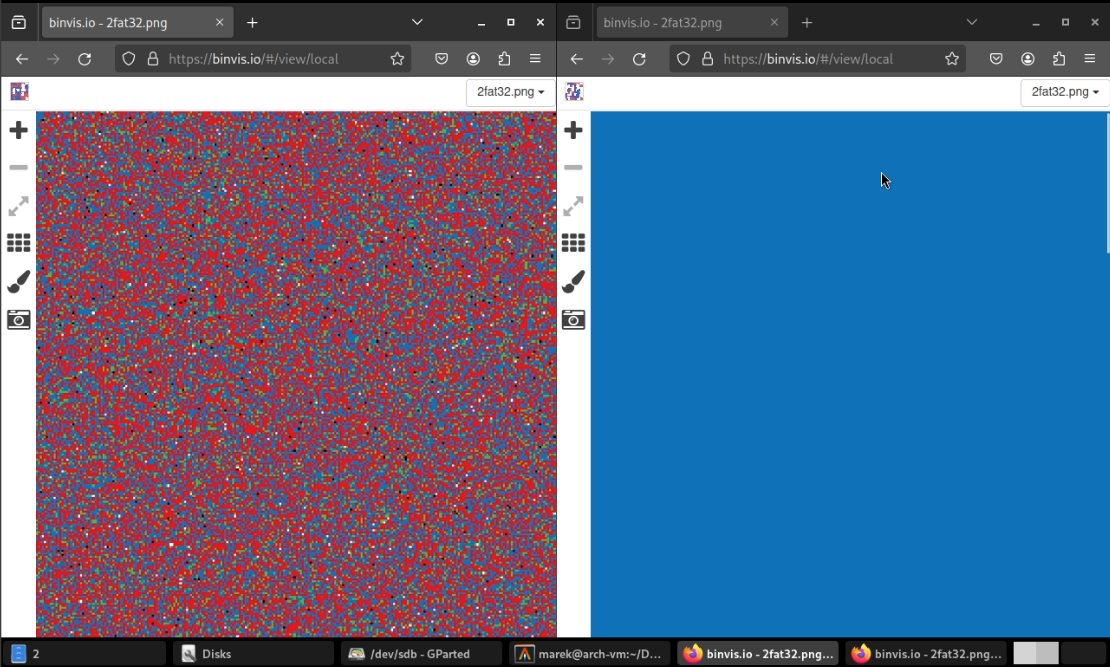
\includegraphics[width=\linewidth]{./images/testdisk_testing/overriden_deleted_file.png}
	\centering
	\captionsetup{justification=centering,margin=2cm}
	\caption{Vizualizácia pomocou binvis.io}
\end{figure}

Na druhej vizualizácii je vidieť kde už pokračujú pozostatky dát z obrázku, pretože nebol prepísaný celý, keďže bol väčší ako textový súbor.

\begin{figure}[H]
	\centering
	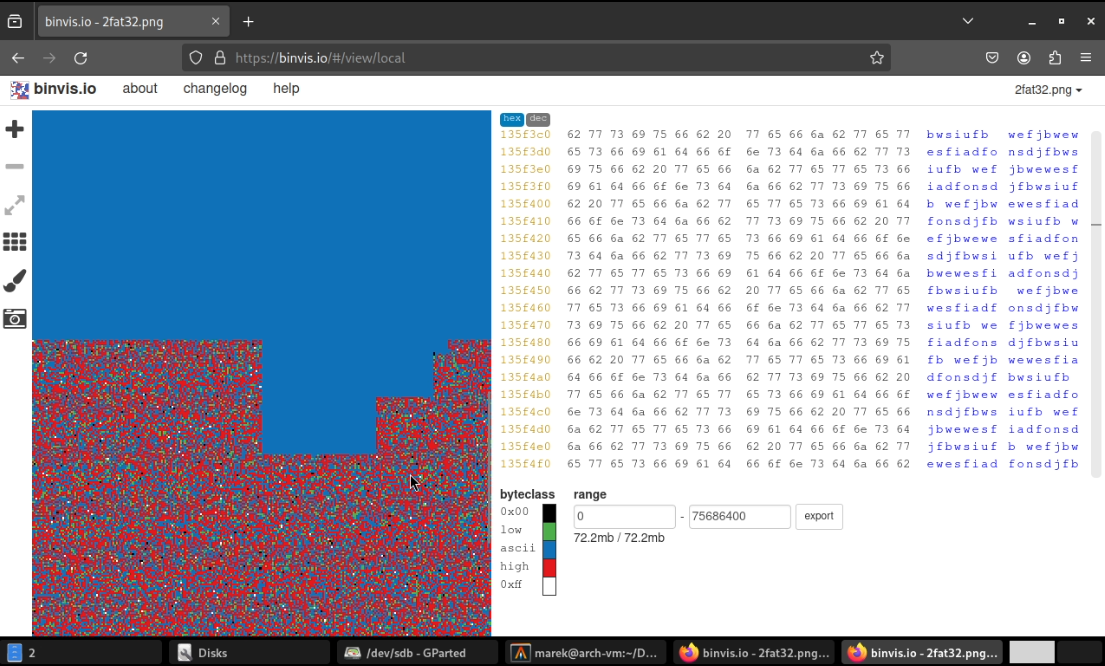
\includegraphics[width=\linewidth]{./images/testdisk_testing/overriden_deleted_file2.png}
	\centering
	\captionsetup{justification=centering,margin=2cm}
	\caption{Vizualizácia pomocou binvis.io --- pozostatky dát}
\end{figure}

Táto skutočnosť nastáva z dôvodu, že pri mazaní súborov z disku sa vymaže iba záznam o súbore a nie sám súbor. V skutočnosti sa ani sám záznam priamo nevymaže ale iba sa označí že na miesto, ktoré mal disk alokovaný pre seba je teraz možné znova zapisovať. Preto je možné dáta z diskov obnoviť ale iba v prípade, že nebudeme zapisovať na daný disk. Keď sa však na miesto zmazaného súboru zapíše iný súbor, tak sa dáta pôvodného súboru prepíšu a týmto sa stane neobnoviteľným.


\subsection{Zmazanie a obnova partícií}
Po predošlom experimentovaní som na záver pomocou programu Gparted vymazal všetky partície.

\begin{figure}[H]
	\centering
	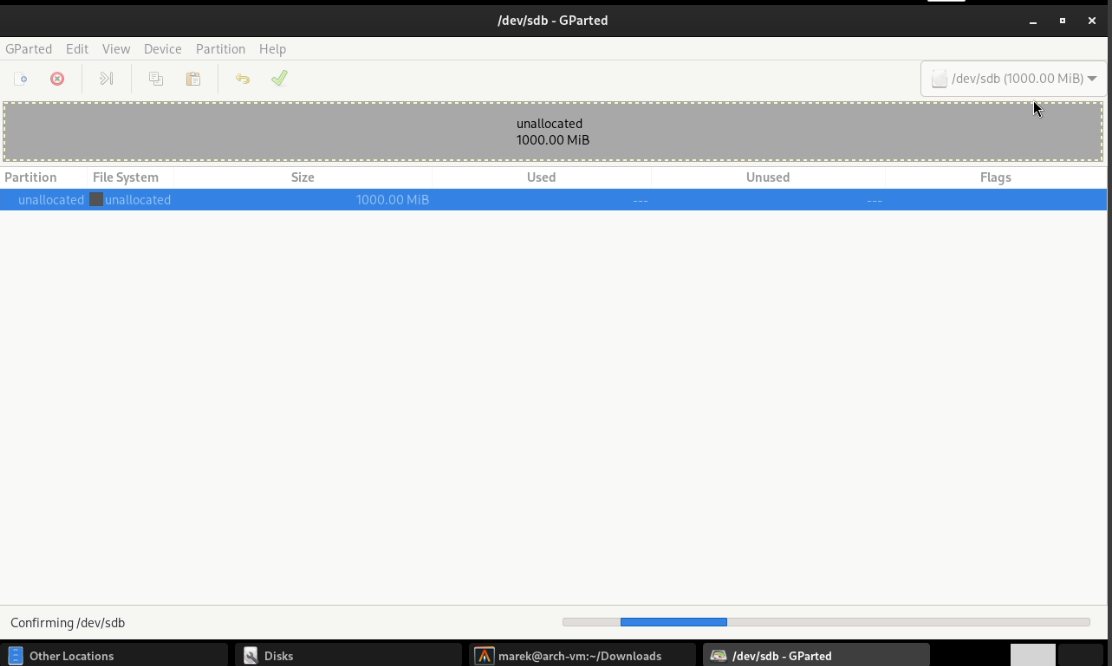
\includegraphics[width=\linewidth]{./images/testdisk_testing/partitions_deletion.png}
	\centering
	\captionsetup{justification=centering,margin=2cm}
	\caption{GParted --- Vymazanie partícií}
\end{figure}

Opät som spustil nástroj testdisk a postupoval podobne ako pri obnove súborov, avšak tentoraz som vybral možnosť ``Analyse'' a nástroj mi zobrazil všetky zmazané partície. Môžeme si všimnúť, že posledná partícia bola označená ako NTFS aj keď bola naformátovaná na exFAT. Testdisk pravdepodobne iba chybne určil typ jej súborového systému. Následne som potvrdil aby sa partície obnovili. Chyba určenia typu pri exFAT nakoniec ničomu nevadila, pretože aplikácia GNOME Disks vedela že ide o exFAT. 

\begin{figure}[H]
	\centering
	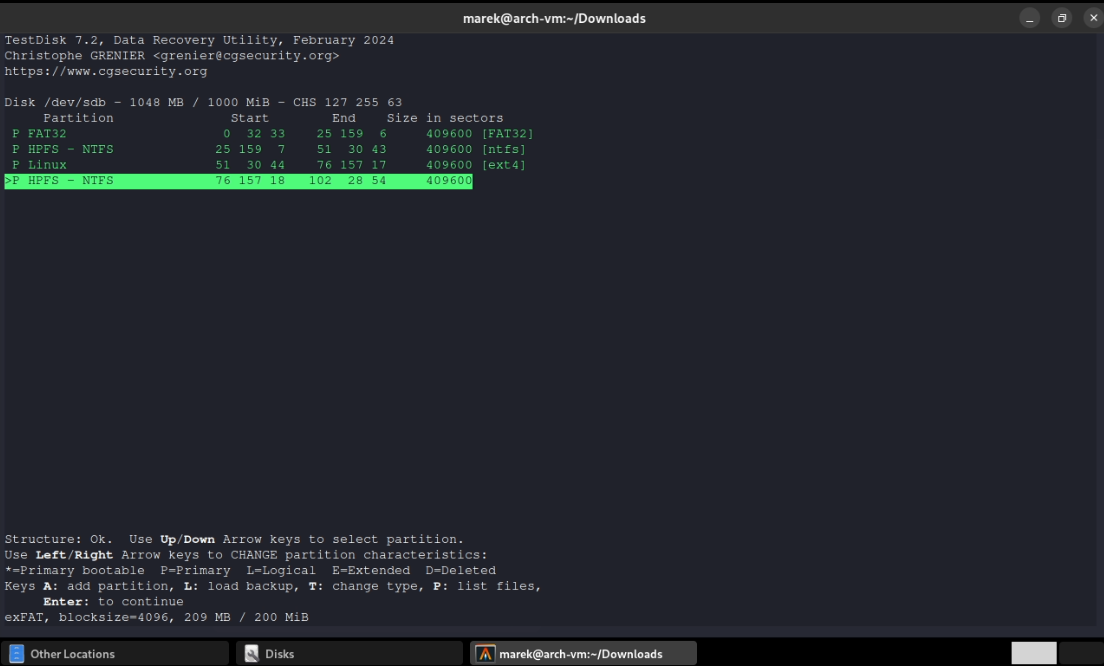
\includegraphics[width=\linewidth]{./images/testdisk_testing/partitions_recovery.png}
	\centering
	\captionsetup{justification=centering,margin=2cm}
	\caption{Testdisk --- obnova zmazaných partícií}
\end{figure}



\section{Výsledky experimentov}
\subsection{Zmazanie súborov}
Pri práci s FAT32 a exFAT neboli problémy a súbor sa mi podarilo v poriadku obnoviť.

V prípado NTFS nastali komplikácie. Testdisk hlásil, že súborový systém je poškodený. Vtedy som zvolil možnosť ``Analyse'', ktorá ho opravila a potom po reštarte VM a spustení testdisku som mohol pokračovať v obnove zmazaných súborov. Pri NTFS sa to riešilo cez inodes a pri obnove bolo treba premenovať súbor aj s koncovkou a nastaviť nad ním vlastníctvo\footnote{ownership}. Táto komplikácia bola pravdepodobne spôsobená tým, že som pracoval na virtuálnom stroji a nie na fyzickom disku. Prípadne preto, že som pracoval na Linuxe a nie na Windows.

\begin{figure}[H]
	\centering
	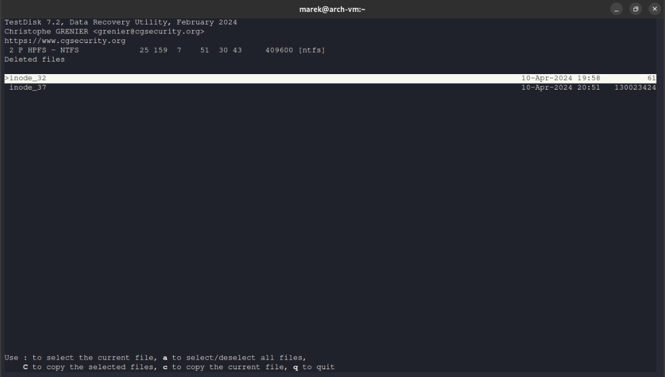
\includegraphics[scale=0.8]{./images/testdisk_testing/testdisk_deleted_file_recovery3.png}
	\centering
	\captionsetup{justification=centering,margin=2cm}
	\caption{Testdisk --- obnova zmazaných súborov --- NTFS}
\end{figure}

Zo súborového systému ext4 sa mi nepodarilo obnoviť súbor pretože ho testdisk nezobrazoval. Neskôr som sa v dokumentácii dočítal, že testdisk podporuje ext2 čo mi však prišlo zváštne. Každopádne som tento proces skúsil na disku, kde bola jedna partícia naformátovaná na ext2 avšak aj v tomto prípade mi zmazaný súbor nezobrazovalo. Pravdepodobne to bolo spôsobené tým, že som pracoval vo virtuálnom prostredí.

V tomto experimentovaní sme používali pevný disk (HDD). Ak by sme však chceli použiť SSD, bolo by treba aby nemalo funkciu TRIM, alebo ju malo vypnutú. Je to z dôvodu že táto funckia pri SSD diskoch zabezpečuje rovnomerné opotrebovanie disku a preto sa dáta ukladajú náhodne na rôzne bunky a nie sekvenčne ako na HDD. To spôsobuje že po zavolaní tejto funkcie sa spustení tzv. garbage collector a naše dáta sa stanú neobnoviteľnými.

\subsection{Prepísanie zmazaných súborov}
Z tohto experimentu nám vyplýva, že ak sa nám niekedy náhodou stane že sme vymazali niečo čo sme nechceli, tak je treba čo najskôr prestať zapisovať na disk. To môžeme docieliť kompletným vypnutím počítača. Ak sa nám podarí zastaviť zápis na disk, tak je veľká šanca že sa nám podarí obnoviť zmazané súbory. Ak však začneme zapisovať na disk, tak je šanca že sa nám nepodarí obnoviť súbory, pretože sa dáta prepíšu.

\subsection{Zmazanie partícií}
Pri obnove zmazaných partícií som nemal žiadne problémy. Testdisk ich zobrazil a následne som ich mohol obnoviť. V prípade, že by som mal dáta na týchto partíciách, tak by som ich mohol obnoviť. Tento proces by bol podobný ako pri obnove zmazaných súborov.

\section{Bezpečné zmazanie dát z disku}
Na bezpečné zmazanie súborov na disku alebo celých partícií vieme použiť príkaz ``shred''. Funguje však iba pre HDD. V prípade SSD nemusí príkaz fungovať vzhľadom na ich mechanizmy rovnomerného opotrebenia. Tieto mechanizmy môžu zabrániť tomu, aby ``shred'' prepísal údaje na mieste, kde má. Hoci neexistuje dokonalé riešenie tohto problému, jedno z riešení je zašifrovanie údajov pred ich vymazaním. Týmto spôsobom budú údaje nečitateľné bez šifrovacieho kľúča aj v prípade ich obnovenia.

Príkaz ``shred'' dokáže prepísať súbor/y náhodnými dátami a použitím daných prepínač si môžeme vybrať koľko krát sa toto prepisovanie udiať. Taktiež si môžeme vybrať aby sa na konci prepísal na samé nuli aby sme zamaskovali stopy po prepísaní. Následne súbor vieme pomocou prepínača aj vymazať.

Ukážka použitia príkazu ``shred'' na súbore ``test.txt'':
\begin{verbatim}
	shred -n 5 -vz test.txt
\end{verbatim}
Prepíšeme daný súbor 5 krát, na konci ho prepíšeme na samé nuly.

Ukážka použitia pre bezpečné zmazanie partície:
\begin{verbatim}
	shred -n 5 -vz /dev/sda
\end{verbatim}

Prepínč ``-n'' určuje koľko krát sa má súbor/partícia prepísať, ``-v'' zobrazuje priebeh (tzv. verbose mode) a ``-z'' prepíše súbor/partíciu na samé nuly.

\section{Záver}
V tejto práci sme sa zaoberali súborovými systémami a nástrojmi na obnovu dát. Na začiatku sme si predstavili súborové systémy NTFS, FAT32, exFAT, ext4 a nástroj testdisk. Taktiež sme sa zaoberali výhodami a nevýhodami každého spomenutého súborového systému. Potom sme sa venovali experimentovaniu s nástrojom testdisk. Vyskúšali sme obnovu zmazaných súborov a partícií. Následne sme sa pozreli na bezpečné zmazanie dát z disku. Na záver môžeme povedať, že nástroj testdisk je veľmi užitočný nástroj na obnovu dát avšak ak sa nám stane situácia, kedy zmažeme dáta, ktoré sme nechceli zmazať, tak je dôležité aby sme čo najskôr prestať zapisovať na disk.

\pagebreak
\bibliography{literatura}
\bibliographystyle{unsrtnat}
\end{document}